\documentclass{article}

% if you need to pass options to natbib, use, e.g.:
%     \PassOptionsToPackage{numbers, compress}{natbib}
% before loading neurips_2021

% ready for submission
\usepackage[preprint]{neurips_2021}
\usepackage{printlen}
\usepackage{pgf}
\usepackage{float}
% to compile a preprint version, e.g., for submission to arXiv, add add the
% [preprint] option:
%     \usepackage[preprint]{neurips_2021}

% to compile a camera-ready version, add the [final] option, e.g.:
%     \usepackage[final]{neurips_2021}

% to avoid loading the natbib package, add option nonatbib:
%    \usepackage[nonatbib]{neurips_2021}

\usepackage[utf8]{inputenc} % allow utf-8 input
\usepackage[T1]{fontenc}    % use 8-bit T1 fonts
\usepackage[colorlinks=true]{hyperref}       % hyperlinks
\usepackage{url}            % simple URL typesetting
\usepackage{booktabs}       % professional-quality tables
\usepackage{amsfonts}       % blackboard math symbols
\usepackage{nicefrac}       % compact symbols for 1/2, etc.
\usepackage{microtype}      % microtypography
\usepackage{xcolor}         % colors

\title{Predicting Telecom Churn\\ and Implications of t-SNE}

% The \author macro works with any number of authors. There are two commands
% used to separate the names and addresses of multiple authors: \And and \AND.
%
% Using \And between authors leaves it to LaTeX to determine where to break the
% lines. Using \AND forces a line break at that point. So, if LaTeX puts 3 of 4
% authors names on the first line, and the last on the second line, try using
% \AND instead of \And before the third author name.

\author{%
  Abhijit Kumar Baruah\\
  Matrikelnummer: 5708583\\
  \texttt{abhijit-kumar.baruah@student.uni-tuebingen.de} \\
  \textbf{Github: }\href{https://github.com/abhijit-baruah/Data_Literacy}{Predicting Telecom Churn}
}

\begin{document}

\maketitle

\begin{abstract}
	This project plans to use the  \href{https://www.kaggle.com/mnassrib/telecom-churn-datasets?select=churn-bigml-80.csv}{Telecom churn dataset} to see how different factors influence customer retainability (or churn). We would also like to see how visual representations using a manifold learning technique like t-SNE could be both beneficial and misleading . We plan to use logistic regression for churn predictions.
\end{abstract}

With the ever-increasing usage of telecom services, service providers want to attract new customers while retaining existing ones (churn rate). A high churn rate adversely affects a company's growth. So, an understanding of the factors that influence churn rates becomes vital. 
\section{Dataset}
The current dataset is from \href{https://www.kaggle.com/mnassrib/telecom-churn-datasets?select=churn-bigml-80.csv}{Kaggle} which originated from the company Orange. The dataset, with $3333$ rows across $21$ variables, contains categorical information regarding customer demographics and types of telecom service plans. Customer usage behaviour was recorded across several numeric variables like number of voice mail messages, total day minutes, total day calls, total day charge, total eve minutes, total eve calls, total eve charge, total night minutes, total night calls, total night charge, total international minutes, total international calls, total international charge and customer service calls. The target variable customer churn is an indicator variable for the customer discontinuing telecom services. The dataset is unbalanced as only $14.49\%$ of the total customers stopped services.

\section{Research Questions}
\begin{itemize}
	\item Which was the most important factor associated with high churn rates?
	\item Is accuracy score always a good measure of a prediction model?
\end{itemize}

\section{Exploratory Analysis}
\subsection{Quantitative Analysis}
At the very outset no missing data was observed. The correlations plot of the numeric variables showed that churn was not the only dependent variable. As could be seen from the correlations plot below, the `charge' variables, such as the \textit{total day charge}, were directly calculated from their corresponding `minutes' variables, i.e. \textit{total day minutes}, making them dependent. Since these dependent variables did not add information towards the target variable, they were dropped. 
\begin{figure}[H]
	\begin{center}
		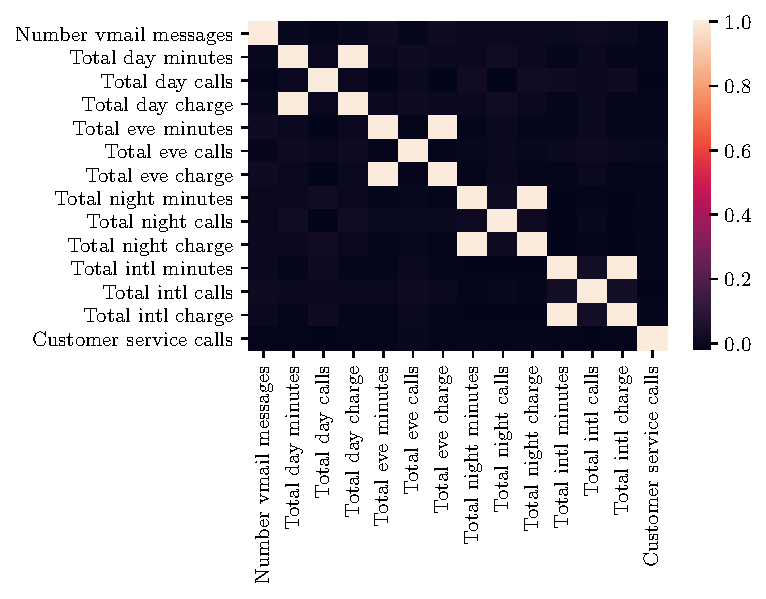
\includegraphics[scale=0.80]{corr.pdf}
	\end{center}
	\caption{Correlations Plot}
\end{figure}

To check for apparent linear or non-linear relationships between the remaining numeric variables, the pairwise scatter plots were plotted as shown below.
\begin{figure}[H]
	\begin{center}
		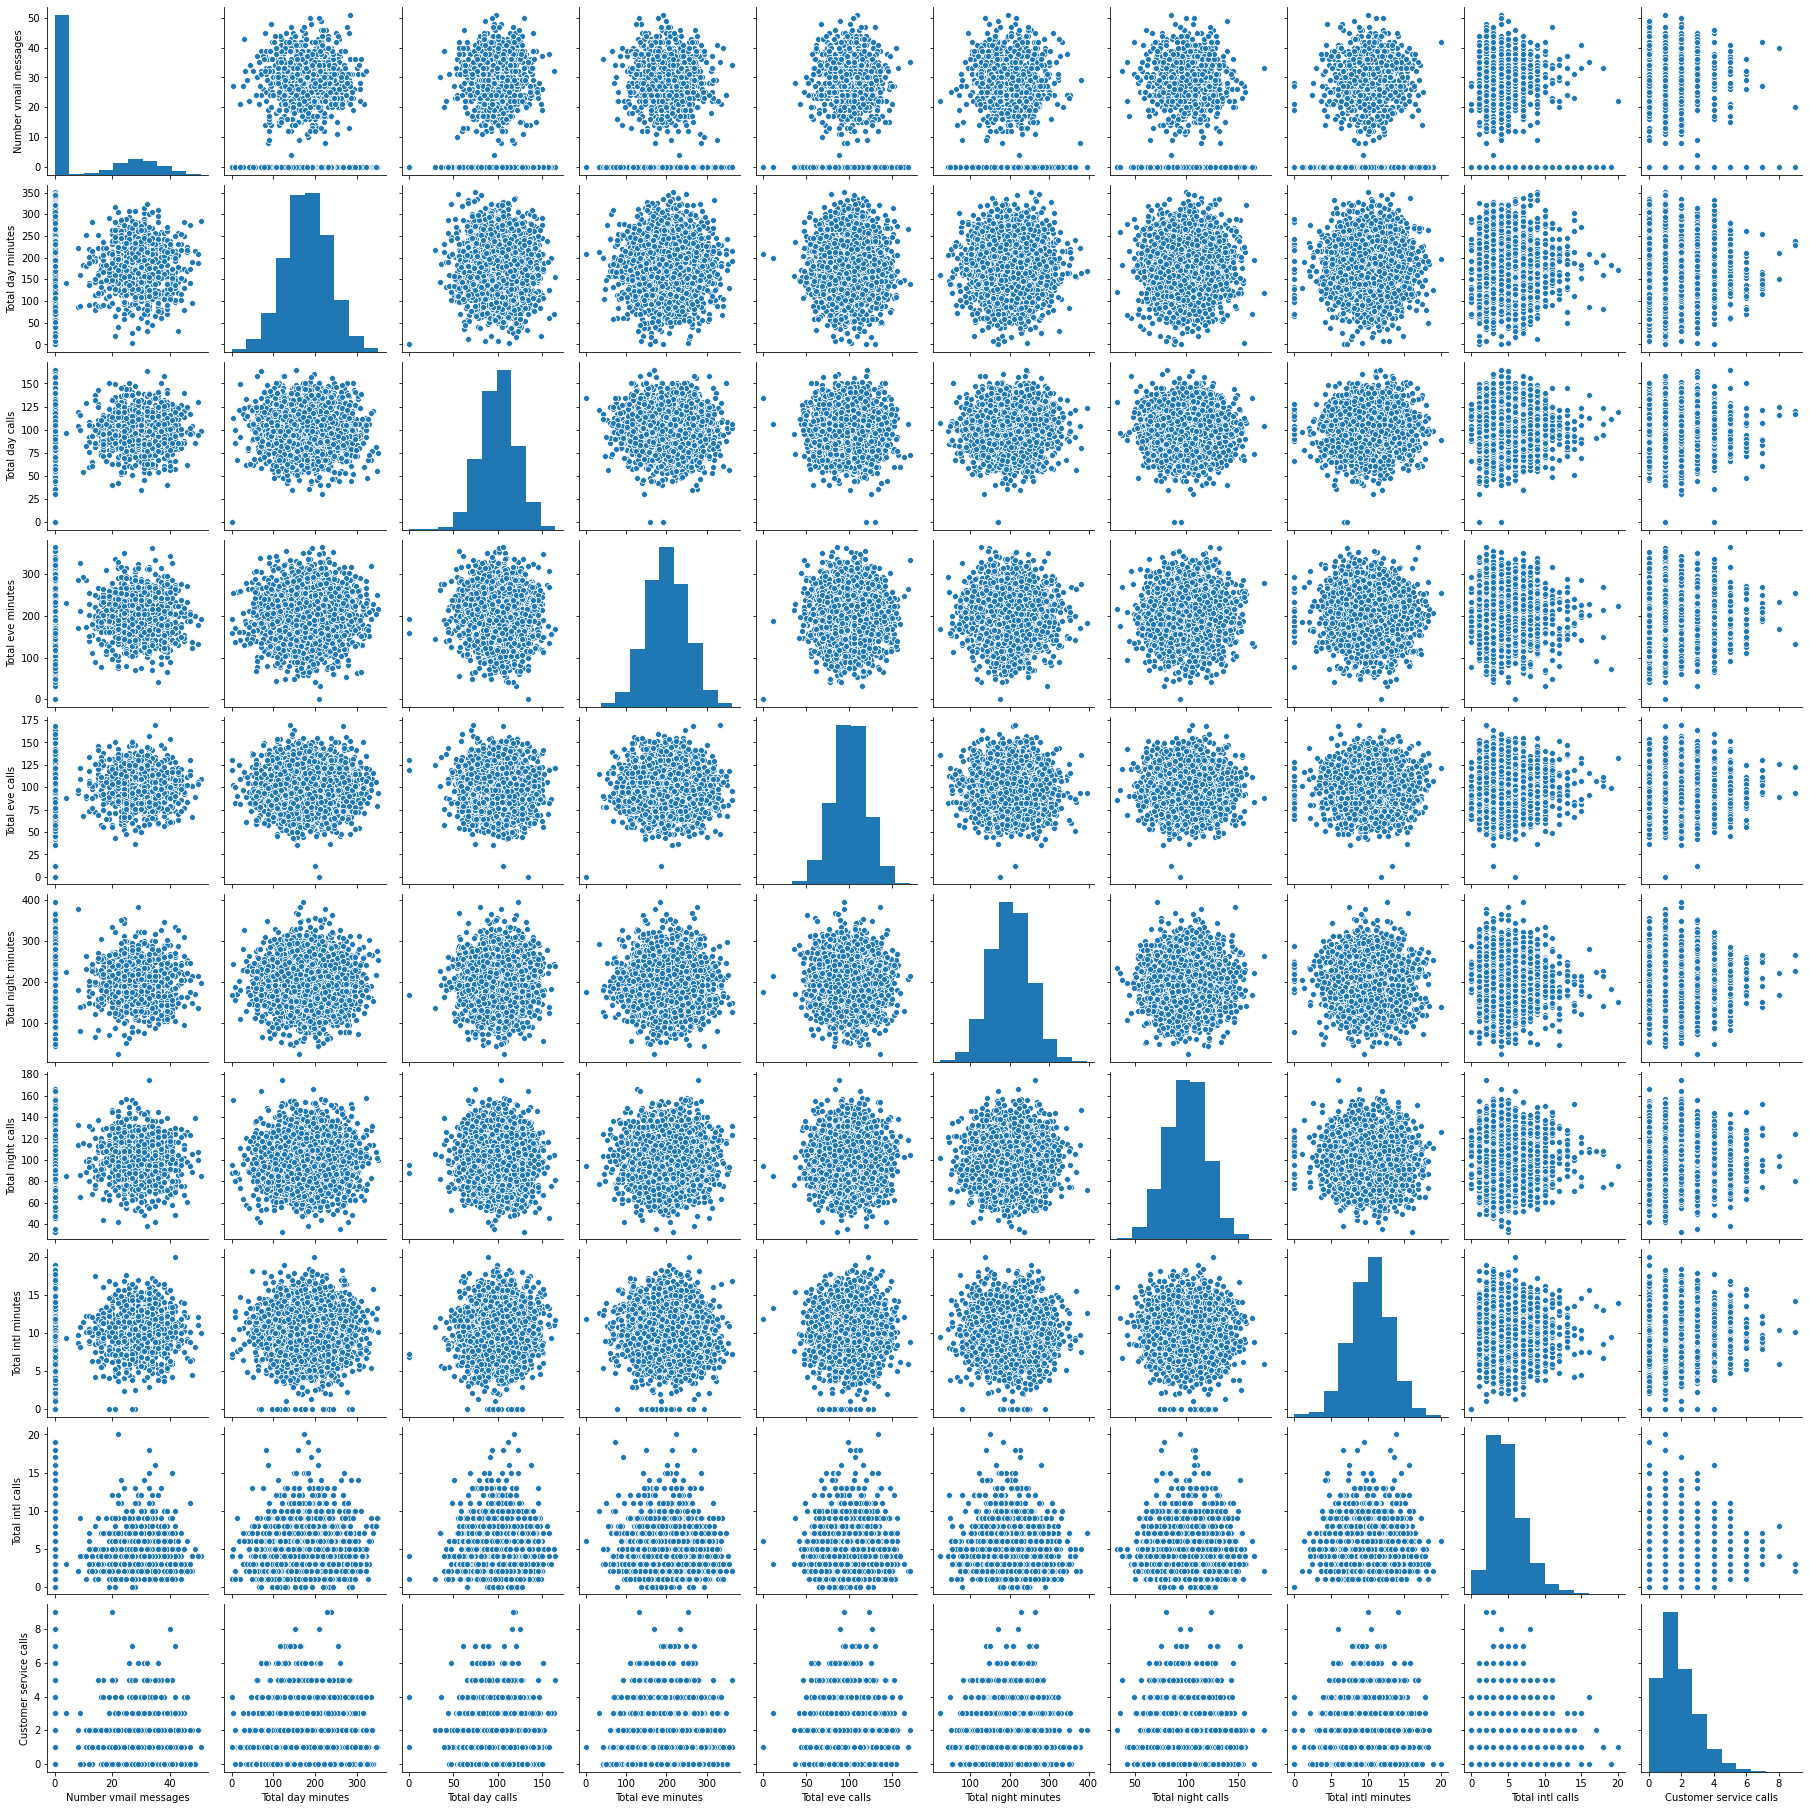
\includegraphics[scale=0.15]{pair.png}
	\end{center}
	\caption{Scatter Plot}
\end{figure}
As expected, no relationships were seen between the remaining independent variables. The distributions along the diagonal did not show any abnormal or unexpected behaviour.

\subsection{Categorical Analysis}

The goal for this section was to undergo a visual exploration of the concentration of churned customers by their choices of service plans, namely the categorical variables \textit{International Plan} and \textit{Voice Mail Plan}.

The current dataset did not have high dimensions. This made it possible to perform a visual analysis, like scatter plot, quite efficiently on the numeric data in the previous section. However, this is not always feasible. In opposing scenarios, the need of hour is dimensionality reduction without significant loss of information about the data. A commonly used dimensionality reduction technique is the Principal Component Analysis (PCA) which suffers from the linearity in its algorithm. This often leads to poor visualization of non-linear manifold structures. So, under the assumption that PCA might not provide clear visualization, the project opted for one of the best known non-linear methods under \textit{Manifold Learning} which is \textit{t-Distributed Stochastic Neighbor Embedding} (t-SNE). Shown below are t-SNE plots with perplexity values of $5, 30$ and $50$. Clusters in \textcolor{red}{red} indicate `No' and those in \textcolor{green}{green} indicate `Yes' to the corresponding categorical variable.
\begin{figure}[H]
	\begin{center}
		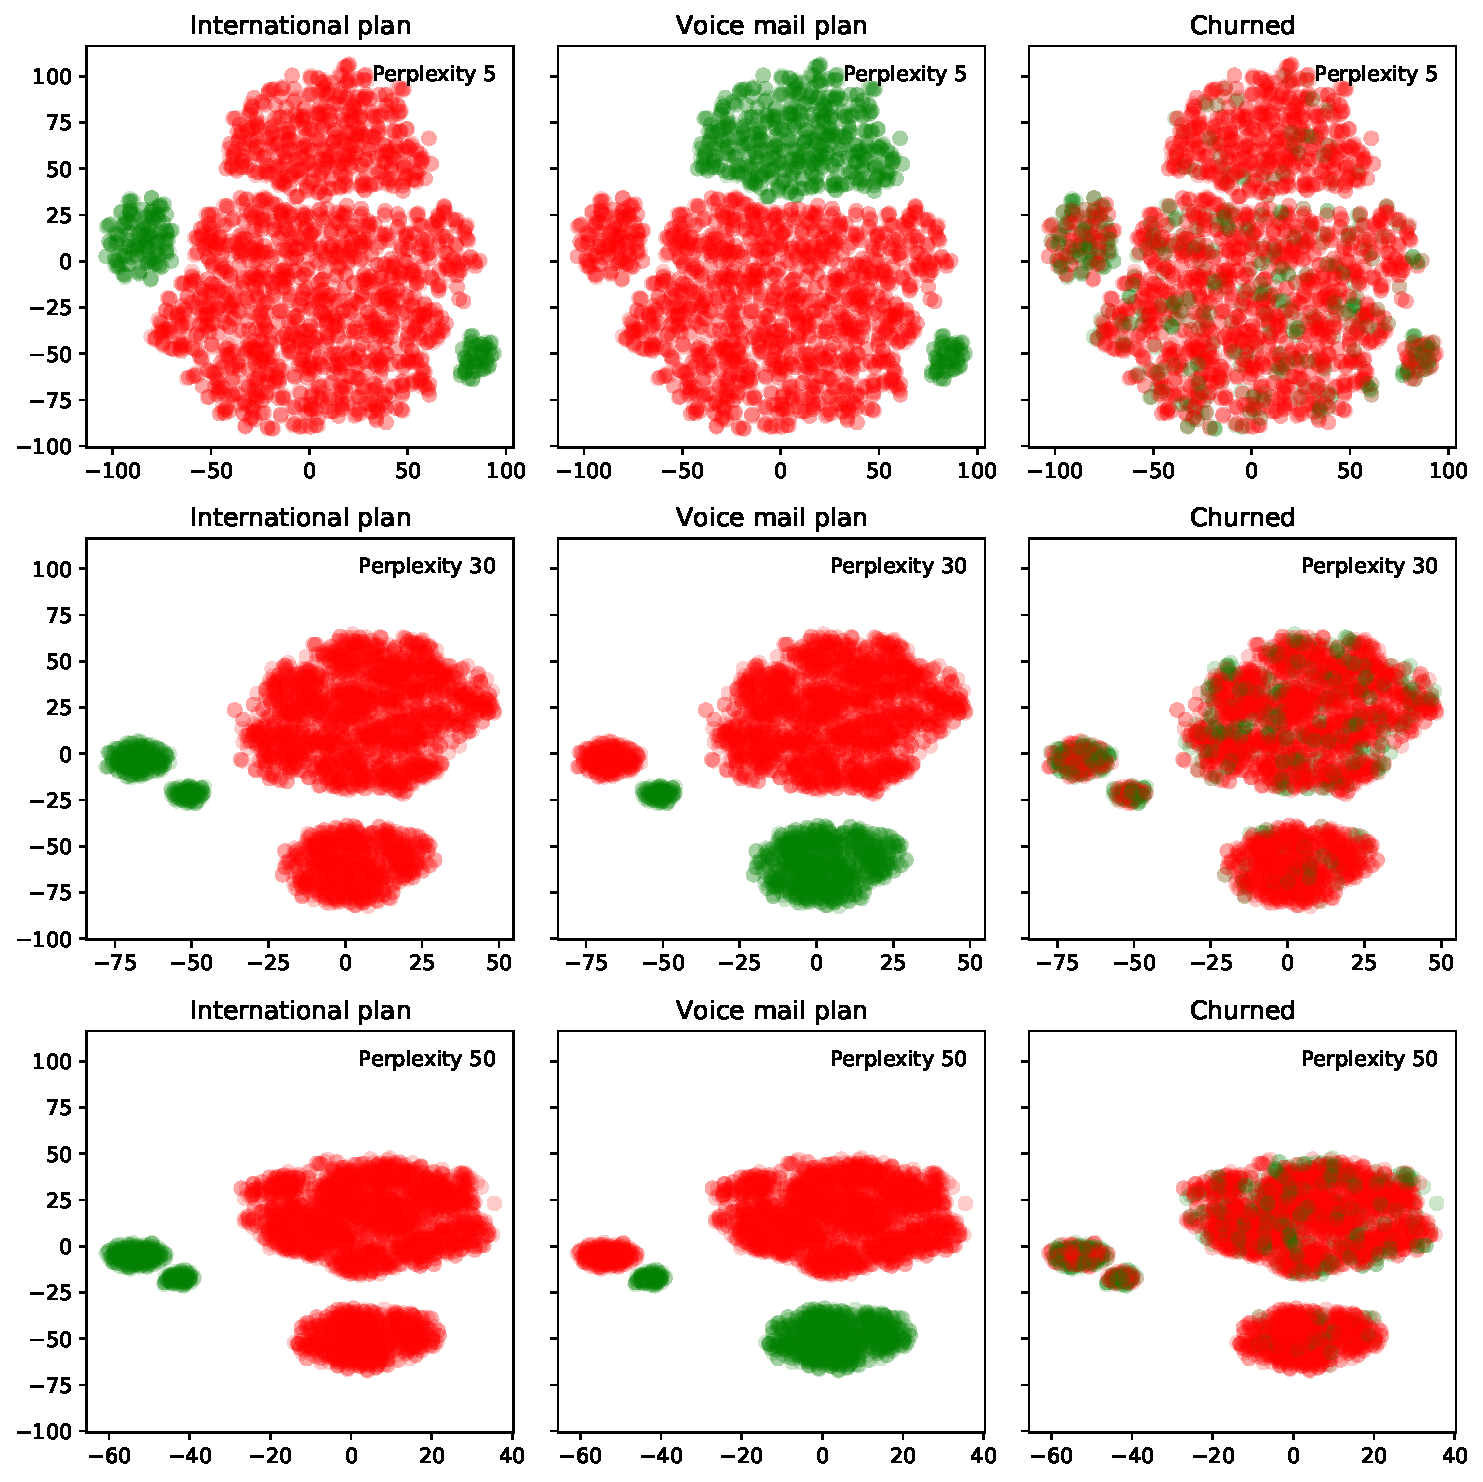
\includegraphics[scale=0.40]{tsne.pdf}
	\end{center}
	\caption{t-SNE Plot}
\end{figure}
\subsection*{Implications of t-SNE:}
\begin{enumerate}
	\item It was evident that the churned customers were concentrated in a few scattered areas in the lower dimensional feature space.
	\item Several discontinuing customers were clustered in areas which represented those with international plans but no voice mail plans.
	\item The perplexity values influence our interpretation of t-SNE plots as higher values lead to merging of clusters. Comments, such as in $(2)$, could not be readily made from, for example, the t-SNE with perplexities of $30, 50$ or higher plot.
	\item Just like any gradient descent based algorithms, t-SNE could also get stuck in local optima especially when causal factors are in higher dimensions.
	\item The basic t-SNE algorithm has high computational complexity due to the nearest neighbor search queries.
	\item In general, far reaching conclusions made from t-SNE needed to be backed with thorough research and formal tests of hypothesis.
\end{enumerate}

\section{Prediction of Churn}
In this final section, logistic regression models were trained to predict churn rates given both the numeric and categorical data (excluding the dependent variables other than Churn). As mentioned earlier, the churn data was unbalanced with the minority class being only $14\%$. So an accuracy score of approximately $86\%$ could be achieved by simply predicting the majority class. The default logistic regression which assumes that both kinds of label error, i.e. false positive (FP) and false negative (FN), had the same cost then would not be the best model to correctly classify the minority class. As such, a weighted logistic regression was also performed assigning majority class a weight of $0.20$ and minority class a weight of $0.80$. So the penalty of wrong prediction of minority class would be $80$ times more severe than wrong prediction of majority class. Moreover, with these class-weight values, the weighted model was expected to perform better then the default one. Below are the confusion matrices and performance metrics comparing the same.
\begin{figure}[H]
	\begin{center}
		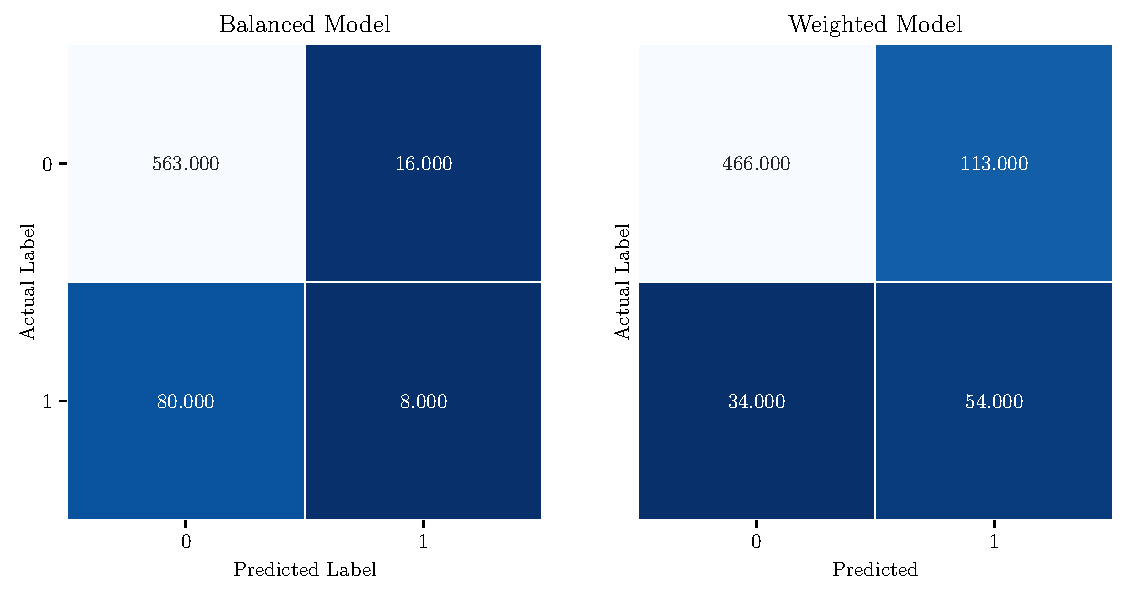
\includegraphics[scale=0.50]{conf_mat.pdf}
	\end{center}
	\caption{Confusion Matrix}
\end{figure}
\begin{table}[ht]
	\begin{center}
	\begin{tabular}{|| c | c | c | c ||}
		\hline
		Model & Accuracy & Area Under Curve & Recall \\ [1ex]
		\hline\hline
		Balanced Logistic Regression & 0.856 & 0.532 & 0.091 \\ 
		\hline
		Weighted Logistic Regression & 0.780 & 0.709 & 0.612 \\ [1ex]
		\hline
	\end{tabular}
\vspace{0.1cm}
\caption{Performance Metrics}
\label{tab:caption}
\end{center}
\end{table}%
Indeed with the weighted Logistic Regression (w-LR), Area-Under-Curve (AUC) increased from $0.532$ to $0.709$. Recall score improved dramatically from $0.091$ to $0.612$. Although the model accuracy decreased in the w-LR model, yet custom weights showed improvements in predicting minority class as expected. This is more crucial in real world cases while making decisions in business and strategy as the minority class of discontinuing customers is the class of interest with the potential of impacting negatively on the company's growth. Model weights suggested that \textit{International Plan} had the greatest influence in customer retention. Customers with the plan were far less susceptible to churning the telecom service then those without. On the other hand, night time call was the least influencing factor towards service discontinuation or retention.

\section*{References}

{
	\small
	
	[1] Kobak, D. \ (2020), \textit{Machine Learning-I Lecture Notes}, University of Tübingen, 2020.
	
	[2] scikit-learn: Machine Learning in Python, accessed on 04 February, 2022, <https://scikit-learn.org/stable/>.
	

}
\end{document}
